%! Author = florian
%! Date = 25.05.23


\section{Alternative Consensus Mechanisms}\label{sec:alternative-consensus-mechanisms}
This section will describe and compare alternative consensus mechanisms.
Around 60\% of the current consensus mechanisms used in blockchains is the POW(Proof-of-Work) consensus mechanism.
As already described in section\ \ref{sec:introduction}, the POW consensus mechanisms requires a miner to solve complex mathematical puzzles in order to create block on the blockchain.
This requires much energy and is therefore bad for the environment.\cite{overview-of-sustainablity-blockchains,moralis-pow-enery-consumption}

By moving to an alternative proof algorithm blockchains could reduce their energy consumption.
This section will describe these alternative consensus mechanisms.\cite{4-ways-to-counter-blockchains-energy-consumption}

\subsection{Proof of Stake}\label{subsec:proof-of-stake}
Proof-of-Stake is the second most used consensus algorithm, next to Proof-of-Work.
Unlike Proof-of-Work, the Proof-of-Stake consensus algorithm does not need miners to create blocks for the blockchain.
Instead, participants, who want to create blocks, have to place a certain amount of the networks tokens as a stake.
These participants are known as validators.
The coins in a stake are locked and cannot be used for transactions.
If a validator wants to access the tokens in their stake, they have to stop being a validator in order to do so.
The amount of blocks they can create is limited by the size of the placed stake.
The creator of a blocks gets the transaction fees associated with the transactions in the block, but no mining reward.\cite{bitpanda-pos}

The nature of Proof-of-Stake is therefore a deterministic algorithm, since the creator of the block is selected by the size their stake.
This can lead to unwanted centralization, since a participant with many tokens has an advantage over participants with only a small amount of tokens.
To prevent the centralization of the network, there are other selection methods, such as:

\begin{itemize}
    \item\textbf{Stationary Time}: Validators are selected based on the amount of time their cryptocurrency has been locked up in the network.\cite{bitpanda-pos}
    \item\textbf{Coin Age}: Validators are selected based on the product of their stake and the amount of time the tokens have been held in the network.\cite{bitflyer-glossary}
    \item\textbf{Randomized Block Selection}: Validators are selected based on a pseudorandom function that combines their stake with other factors such as the hash of the previous block.\cite{cryptonews-pos}
\end{itemize}

\subsection{Proof of Time and Space}\label{subsec:proof-of-time-and-space}
Another alternative consensus mechanism is Proof-of-Space-and-Time(PoST).
It requires participants to use storage space to validate transactions.
It is supposed to be more energy efficient than Proof-of-Work and Proof-of-Stake.

The greater the amount of storage space allocated by a node operator on their hard drive, the increased likelihood of finding a matching hash value from a predetermined list.
This, in turn, enhances their chances of winning the mining reward.
This requires large amount of free space on a hard-drive, but does not need much energy to create new blocks.

In more details, Proof-of-Space-and-Time consists of two different consensus mechanisms, that are combined.
First, Proof-of-Space, this is the reserved hard-drive space for mining blocks.
Second, Proof-of-Time, this requires a small delay between block validation using a verifiable delay function.
This delay is to stop miners from getting additional rewards when mining with multiple machines in parallel on one node.
It is still possible for miners to run multiple nodes.\cite{supraoracles-post}

\subsubsection{Pros and Cons of Proof of Space and Time}
As already mentioned PoST is more energy efficient as it uses unused storage space rather than computation.
The hardware requirements to run a validator node is also lower, as it only requires free storage space.

One major disadvantage of PoSt its increased wear on HDDs and SSDs.
It can reduce the shelf life of a hard drive to only 40 days rather than the usual shelf life of a decade.
This also means, while PoST itself requires less energy, it may not be an eco-friendly solution, since validators will have to buy new hard drives more frequently and produce more waste.
Compared to the lifespan of a gpu that is used to mine cryptocurrencies, which is about three to five years, this is way less.
So while being more energy efficient, PoST is definitely not better for the environment.\cite{euronews-chia, devicetest-gpu-lifespan, supraoracles-post}

\subsection{Proof of Authority}\label{subsec:proof-of-authority}
The Proof-of-Authority consensus mechanism is very different to the other consensus algorithms already described in this section.
It is suitable for private blockchains.
In Proof-of-Authority not everybody can be a validator.
The validators are preselected based on their reputation, instead of using a stake or time and space.
To become a validator, the candidates identity has to be checked, and the candidate has to be willing to stake money and/or their reputation.
Usually, there should be a rigorous selection process to filter out questionable candidates.\cite{coindesk-poa}

\subsubsection{Pros and Cons of Proof of Authority}
There are multiple pros and cons on Proof-of-Authority.
An advantage of a blockchain based on Proof-of-Authority is that it can execute more transactions per second by not having to calculate a Proof-of-Work everytime a validator builds a block.
Blockchains using Proof-of-Authority are also better secured against 51\% attacks, since the validators are all highly vetted.
Validators also do not need special hardware to build blocks compared to Proof-of-Work or Proof-of-Time-and-Space as mentioned in\ \ref{subsec:proof-of-time-and-space}.

A disadvantage would be the centralization of the blockchain, by having to check and identify each potential validator not every participant in the blockchain can become one.
Therefore, the blockchain loses the aspect of being decentralized as being show in figure\ \ref{fig:centralization-of-proof-of-authority}.
One key aspect of blockchains is their immutability.
This makes blockchains resilient to censorship and the blockchain is available to everyone.
By centralizing the validators the blockchain loses these abilities.
It is easier to block a specific participant  or manipulate the blockchain if the validators wish to do so.

Since the validator nodes are publicly known they are vulnerable to manipulation themselves.
An outside actor could try to influence validators to act in a dishonest or destructive way.\cite{insidecrypto-poa,coindesk-poa}

\begin{figure}[h]
    \centering
    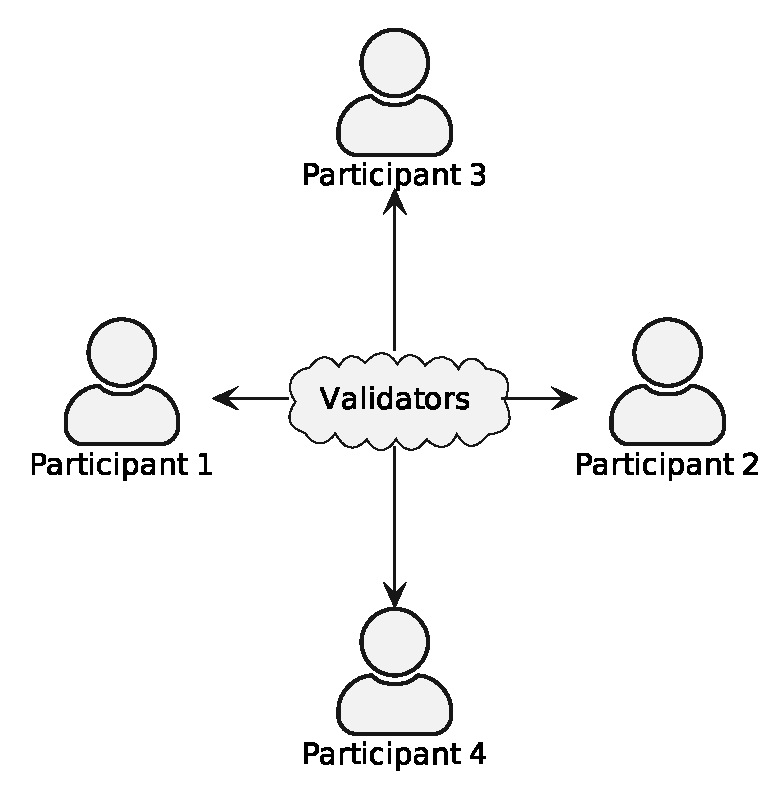
\includegraphics[scale=0.5]{img/proof-of-authority-0}
    \caption{Centralization of Proof of Authority}
    \label{fig:centralization-of-proof-of-authority}
\end{figure}

